\subsection{Work-Effort (LSODA, BDF, Radau)}

Figure \ref{fig:work-effort} plots the trade-off between execution time and \(L_2\) error for the LSODA, BDF, and Radau solvers using sparse Jacobians at a fixed grid resolution of \(N_x = 1000\). The solver tolerances range from \(10^{-2}\) to \(10^{-10}\). The remaining test parameters are fixed at \(p = 2.5\), \(\varepsilon = 10^{-6}\), and \(T=0.05\).

LSODA consistently exhibits the most favorable performance curve in this test. At the tightest tolerance (\(10^{-10}\)), it reaches an \(L_2\) error of \(1.67 \times 10^{-10}\) in just 0.40 seconds. BDF takes 6.39 seconds to hit a similar error margin (\(4.05 \times 10^{-10}\)). Both solvers show predictable log-linear scaling, where tightening the tolerance reliably decreases the error at the expected cost of execution time.

Radau, however, scales anomalously at loose tolerances. At \(10^{-2}\), its execution time spikes to 120.3 seconds. The solver forces hundreds of thousands of function evaluations and overshoots the requested tolerance, landing at an error of \(8.83 \times 10^{-6}\). This behavior suggests that Radau may encounter difficulties with step-size selection or nonlinear convergence at loose tolerances under this specific system stiffness. Once the tolerance is tightened to \(10^{-6}\) and below, Radau's scaling behavior appears to stabilize. It ultimately achieves the lowest absolute error in the suite (\(1.94 \times 10^{-13}\) at \(10^{-10}\) tolerance), but requires 8.65 seconds to do so. Overall, LSODA appears to provide the most practical balance of speed and precision across the tested parameter space.

\begin{figure}[H]
  \centering
  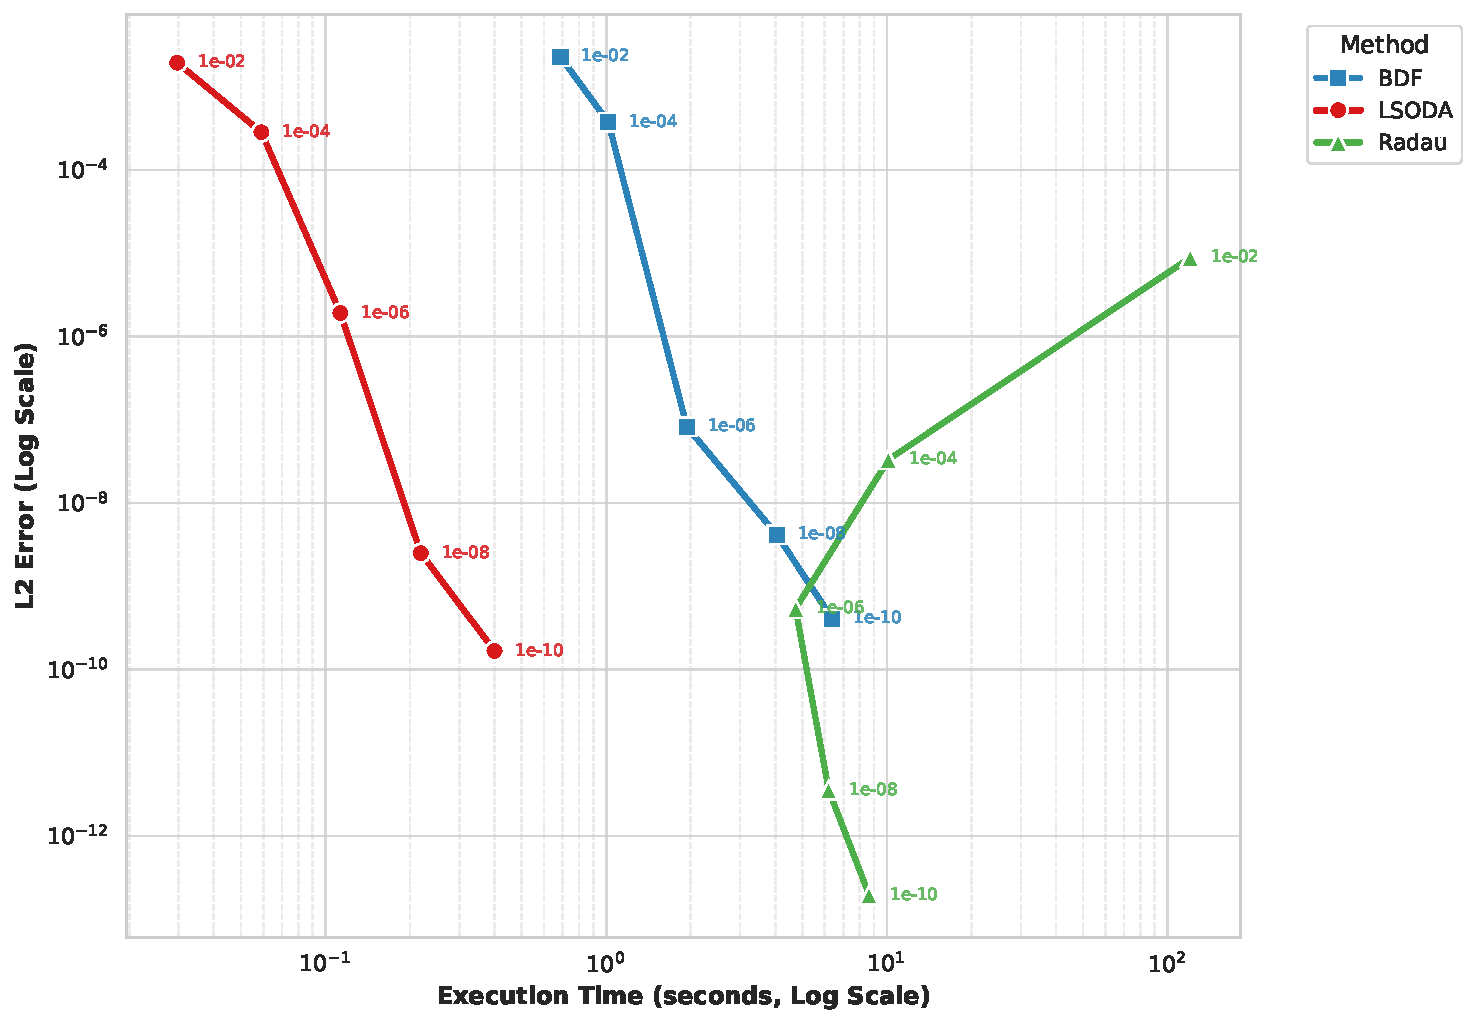
\includegraphics[width=\textwidth]{images/work_effort.pdf}
  \caption{Work-effort diagram illustrating the trade-off between \(L_2\) error and execution time across solver tolerances (\(10^{-2}\) to \(10^{-10}\)) for LSODA, BDF, and Radau.}
  \label{fig:work-effort}
\end{figure}
